\documentclass[../../ASSD_TP1_G7.tex]{subfiles}
\begin{document}
\chapter*{Muestreo sub-Nyquist}
El muestreo sub-Nyquist se utiliza para se\~nales acotadas en banda con el espectro fuera de la Banda base. Para analizar este tipo de muestreo se utilizo una se\~nal AM, ya que su espectro coincide con las característica deseada.
\begin{equation}
X_c=A_{Max}[\frac{1}{2}cos(2\pi (1.8 f_{in})t)+cos(2\pi (2 f_{in})t)+cos(2\pi (2.2 f_{in})t)]
\end{equation}\label{eq:inputSignlan}

Donde $f_{in}= 36KHz$, entonces la frecuencia de la portadora es $72KHz$ y la modulada $7.2KHz$.
\section*{Rango de frecuencia de sampleo}
Definiendo $B$ al ancho de banda de la se\~nal y $f_c$ a la frecuencia central del espectro. El rango de frecuencias de sampleo $(f_s)$ es:
\begin{equation}
f_{sMIN}=\frac{2f_c + B}{m+1} < \frac{2f_c - B}{m} = f_{sMAX}
\end{equation}
Donde $m$ son las repeticiones del espectro. Conociendo $f_{in}$ y la se\~nal AM, $B=14.4KHz$ y $f_c=72KHz$.

\begin{table}[htbp]
\begin{center}
\begin{tabular}{|l|l|l|}
\hline
$m$ & $f_{sMIN}$ & $f_{sMAX}$  \\
\hline \hline
2 & $52.8KHz$ & $64.8KHz$ \\ \hline
3 & $39.6KHz$ & $43.2KHz$ \\ \hline
4 & $31.7KHz$ & $32.4KHz$ \\ \hline
\end{tabular}
\caption{Frecuencias de Sampleo}
\label{tabla:fsamp}
\end{center}
\end{table}
Para $m$ mayores, $f_{sMIN}>f_{sMAX}$.

\section*{Mediciones}
Las mediciones se realizaron para el caso de $m=2$.

Utilizando la frecuencia de sampleo m\'inima (figuras \ref{fig:subnyq_lla_fmin} y \ref{fig:subnyq_syh_fmin}), se observa que las dos r\'eplicas del espectro original (en verde y rojo) est\'an lado a lado. El pico de frecuencia m\'axima de la repetici\'on verde se encuentra superpuesto con el pico de frecuencia m\'inima de la repetici\'on roja, por lo que no se pueden diferenciar en el diagrama espectral. En consecuencia, entre ambas repeticiones deber\'ian medirse 5 picos. 

En las mediciones, tanto en el sample and hold como en la llave anal\'ogica, los espectros de las repeticiones (en rojo y verde) no se distinguen claramente entre s\'i. Una posible explicaci\'on es que la frecuencia de sampleo haya sido menor a la m\'inima por un error en el oscilador, y por lo tanto hayan quedado superpuestos. Tambi\'en se observa fuga espectral en ambos casos. En el sample and hold, esta fuga se encuentra m\'as distribuida que en la llave anal\'ogica, donde se ve claramene un pico tanto en la simulaci\'on como en la medici\'on a $f\approx 55KHz$.

\begin{figure}[H]
\centering
\subcaptionbox{Simulación}
{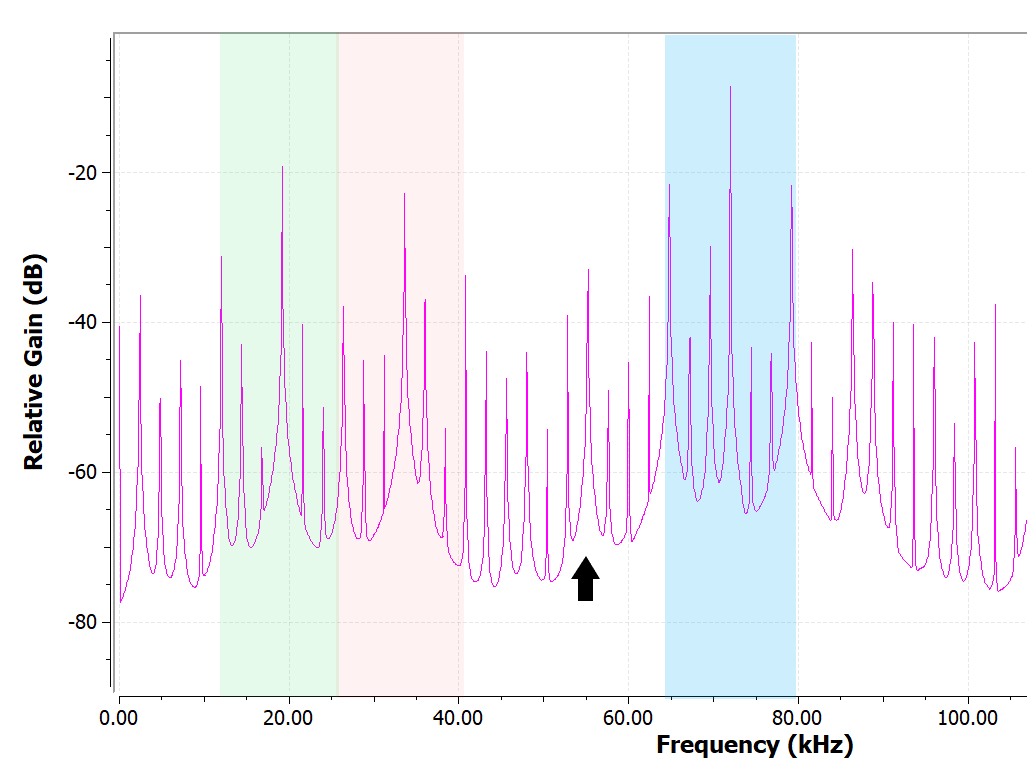
\includegraphics[width=0.6\textwidth]{figures/simpto_8_llave_52,8khz_espectro.png}}
\subcaptionbox{Medición}
{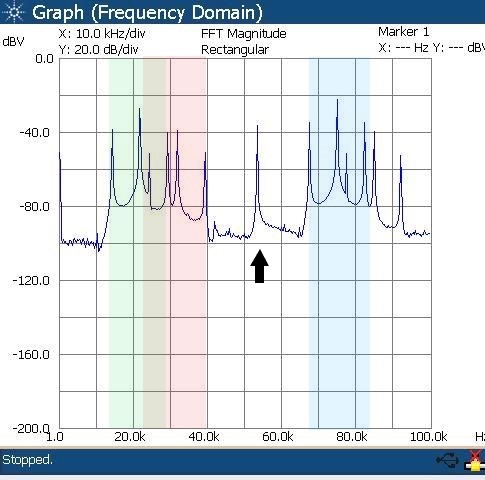
\includegraphics[width=0.32\textwidth]{figures/lla_fmin.jpeg}}
\caption{Frecuencia sampleo mínima(52.8KHz), simulación y medición. Se\~nalado en negro, la frecuencia en la que se encuentra mayor fuga espectral.}
\label{fig:subnyq_lla_fmin}
\end{figure}

\begin{figure}[H]
\centering
\subcaptionbox{Simulación}
{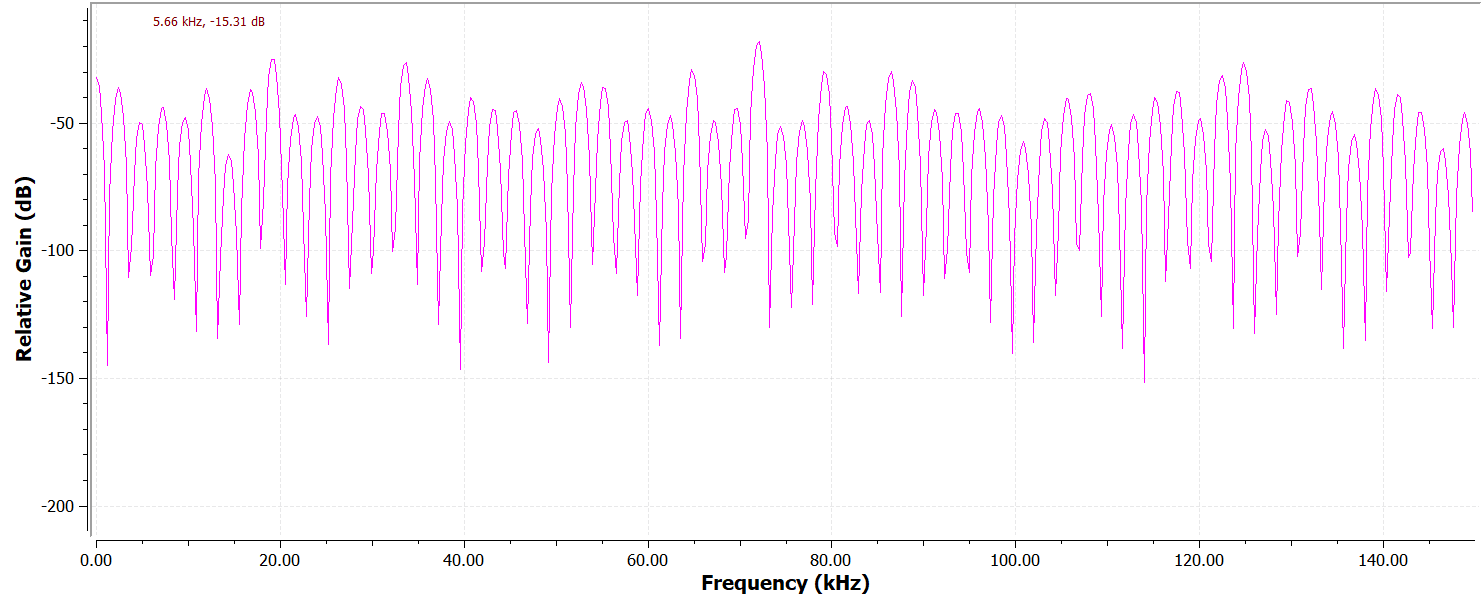
\includegraphics[width=0.6\textwidth]{figures/simpto_8_syh_52,8_espectro.png}}
\subcaptionbox{Medición}
{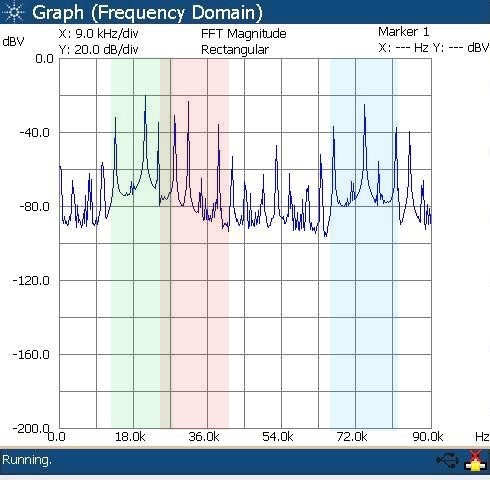
\includegraphics[width=0.32\textwidth]{figures/syh_fmin.jpeg}}
\caption{Frecuencia sampleo mínima(52.8KHz), simulación y medición}
\label{fig:subnyq_syh_fmin}
\end{figure}


Con la frecuencia de sampleo media (figuras \ref{fig:subnyq_lla_fmed} y \ref{fig:subnyq_syh_fmed}), tanto el espectro original (en celeste) como las dos repeticiones (en verde y rojo) se encuentran separados, por lo que no hay picos superpuestos. En consecuencia, 9 picos deber\'ian ser visibles. 

En las mediciones se identifican con claridad los 9 picos, m\'as algunos extras que se atribuyen a la fuga espectral.

\begin{figure}[H]
\centering
\subcaptionbox{Simulacion}
{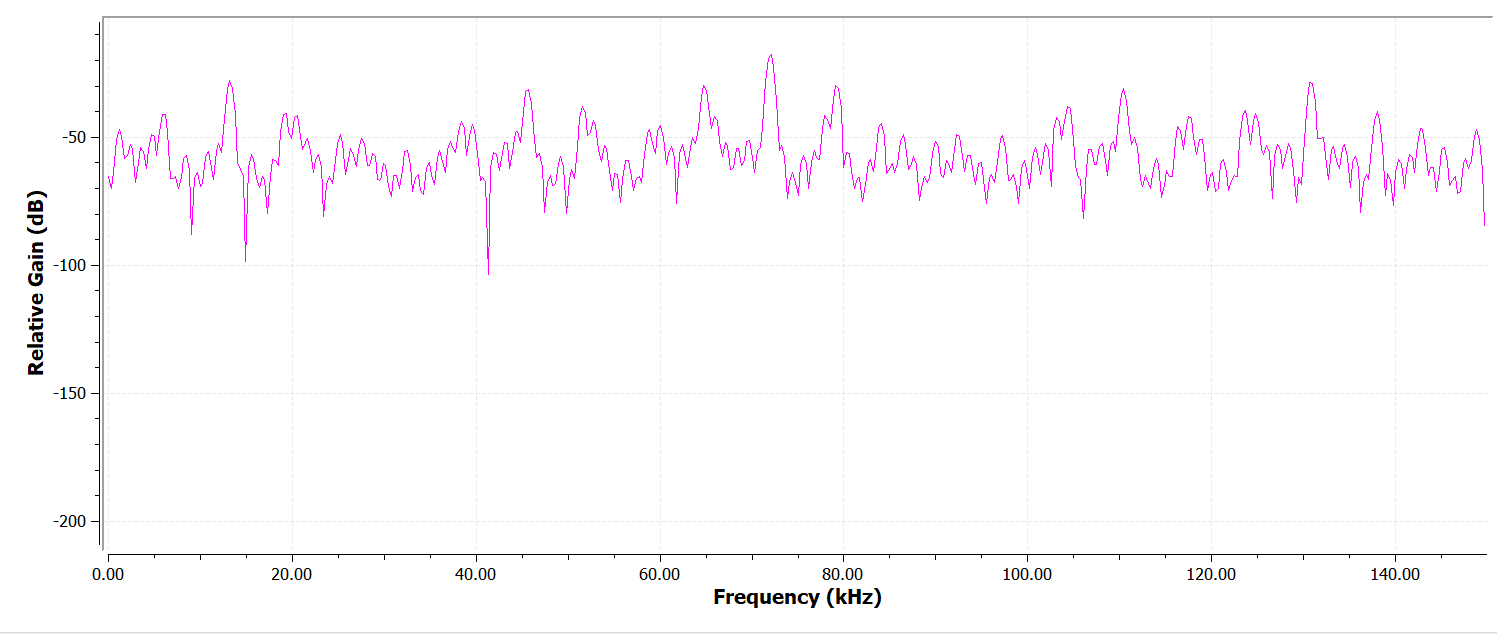
\includegraphics[width=0.6\textwidth]{figures/simpto_8_llave_58,8_espectro.png}}
\subcaptionbox{Medicion}
{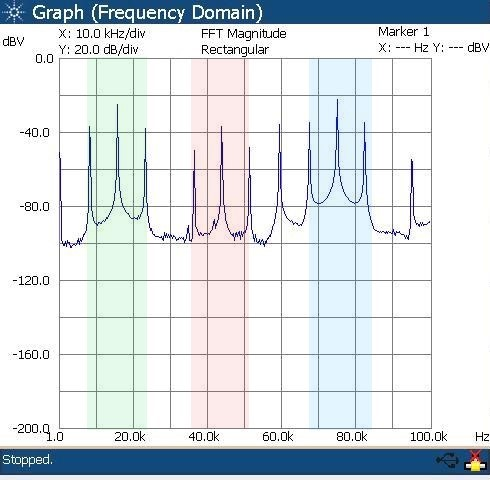
\includegraphics[width=0.32\textwidth]{figures/lla_fmed.jpeg}}
\caption{Frecuencia sampleo media(58.8KHz), simulación y medición}
\label{fig:subnyq_lla_fmed}
\end{figure}



\begin{figure}[H]
\centering
\subcaptionbox{Simulacion}
{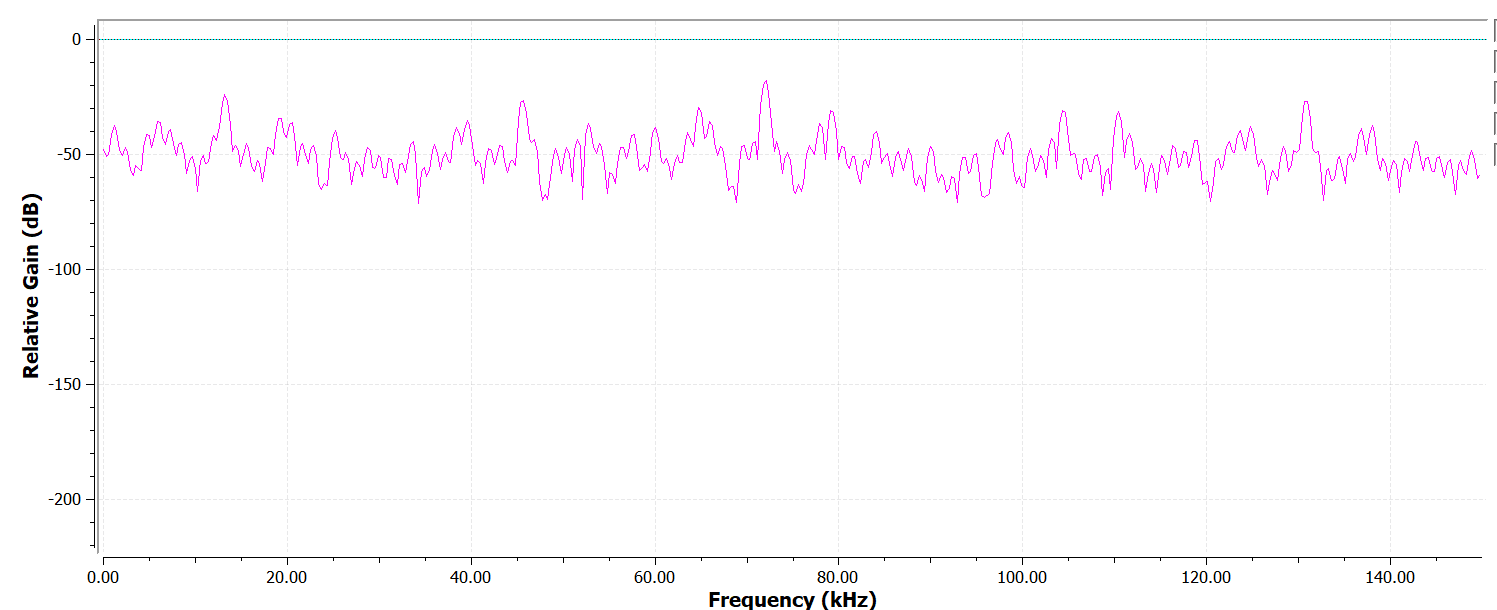
\includegraphics[width=0.6\textwidth]{figures/simpto_8_syh_58,8_espectro.png}}
\subcaptionbox{Medicion}
{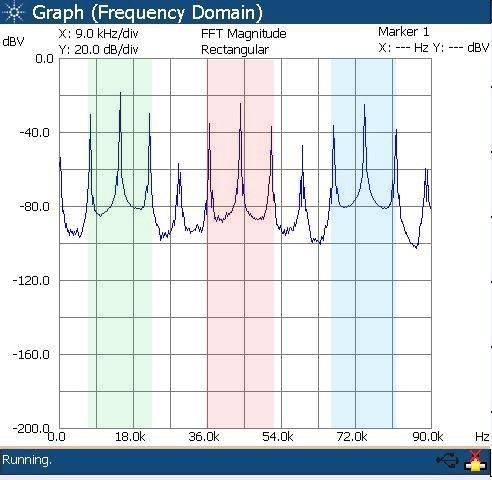
\includegraphics[width=0.32\textwidth]{figures/syh_fmed.jpeg}}
\caption{Frecuencia sampleo media(58.8KHz), simulación y medición}
\label{fig:subnyq_syh_fmed}
\end{figure}


Si la frecuencia de sampleo es la m\'axima, (figuras \ref{fig:subnyq_lla_fmax} y \ref{fig:subnyq_syh_fmax}), el pico superior de la repetici\'on roja coincide con el pico inferior de el espectro original, por lo que se deber\'ian observar 9 picos, 2 de los cuales son muy cercanos. 
Es posible que se superpongan, en cuyo caso se ver\'ian 8. 
Este fue el caso de la simulaci\'on del sample and hold. 
En la simulaci\'on de la llave anal\'ogica, no se distinguen claramente los picos de la repetici\'on de frecuencia m\'as alta (en rojo).

En ambas mediciones se identifican 9 picos, no 8, m\'as picos extras, nuevamente atribuidos a la fuga espectral.

\begin{figure}[H]
\centering
\subcaptionbox{Simulación}
{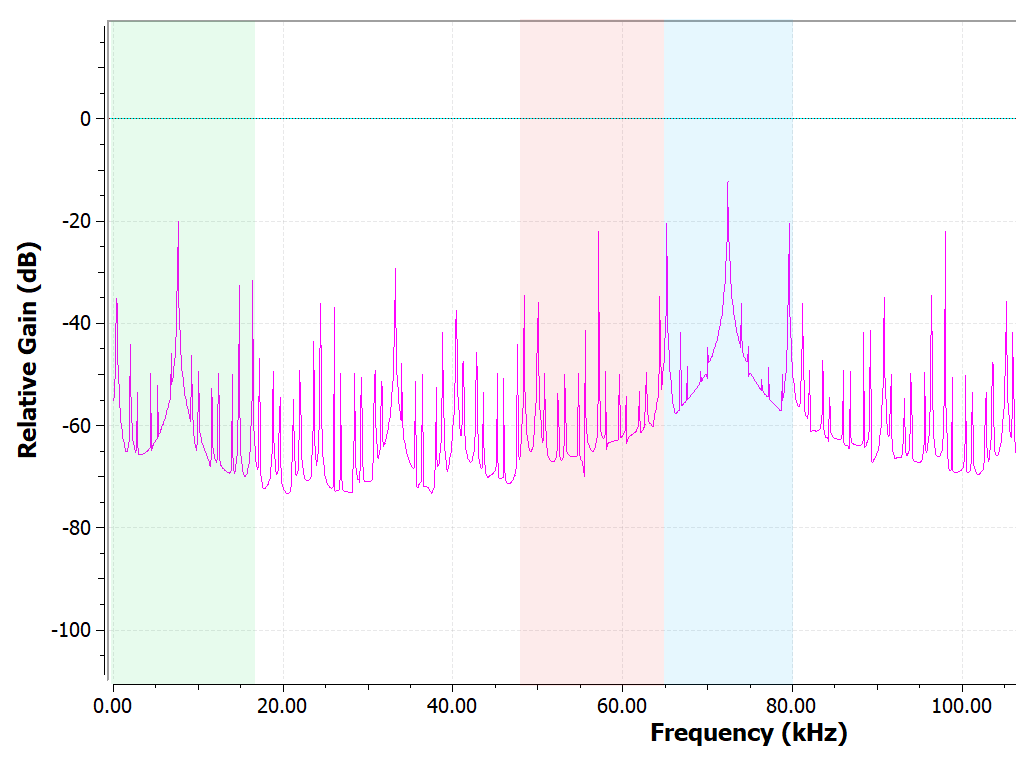
\includegraphics[width=0.6\textwidth]{figures/simpto_8_llave_64,8khz_espectro.png}}
\subcaptionbox{Medición}
{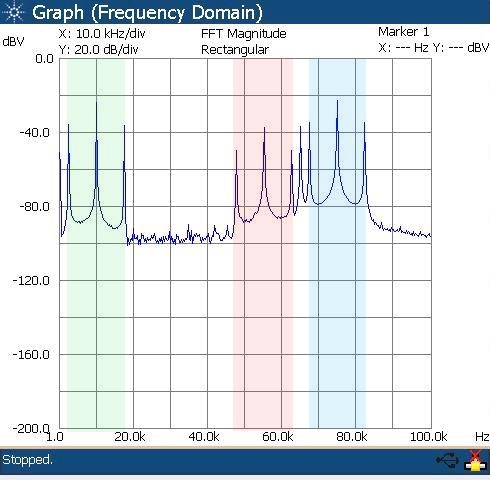
\includegraphics[width=0.32\textwidth]{figures/lla_fmax.jpeg}}
\caption{Frecuencia sampleo maxima(64.8KHz), simulación y medición}
\label{fig:subnyq_lla_fmax}
\end{figure}

\begin{figure}[H]
\centering
\subcaptionbox{Simulación}
{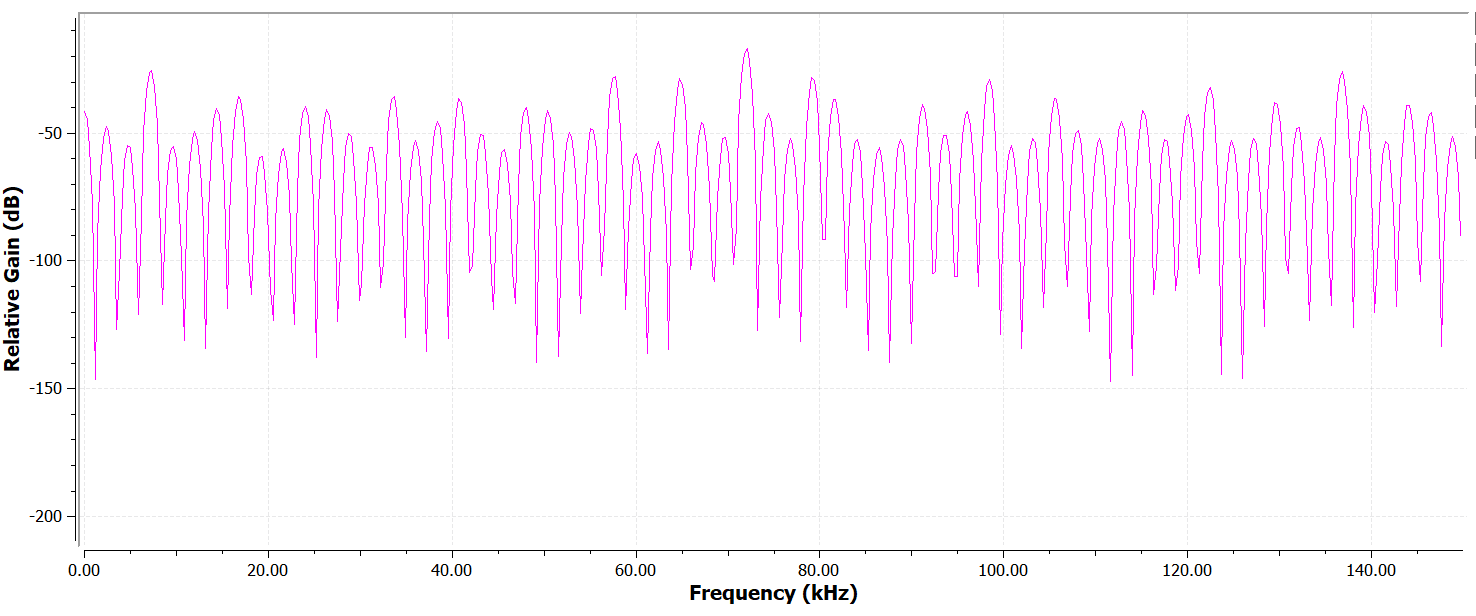
\includegraphics[width=0.6\textwidth]{figures/simpto_8_syh_64,8_espectro.png}}
\subcaptionbox{Medición}
{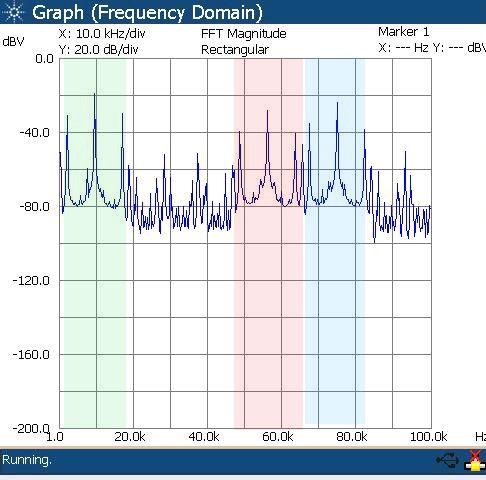
\includegraphics[width=0.32\textwidth]{figures/syh_fmax.jpeg}}
\caption{Frecuencia sampleo maxima(64.8KHz), simulación y medición}
\label{fig:subnyq_syh_fmax}
\end{figure}


\subsection*{Recuperación de la se\~nal}
Se intento recuperar la se\~nal proveniente de la llave analógica, para ello se conecto el filtro recuperador. Se obtuvo la siguiente medición:

\begin{figure}[H]
  \centering
   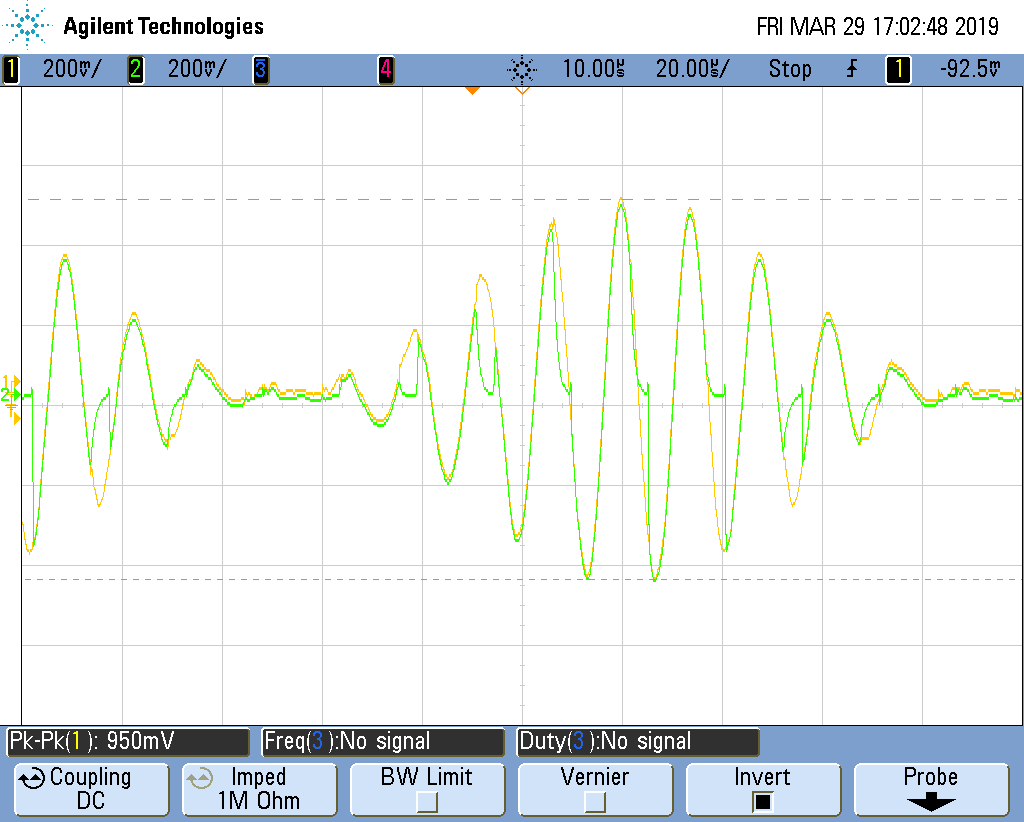
\includegraphics[width=0.7\textwidth]{figures/lla_8_1.png}
  \caption{Recuperación de la se\~nal. Canal amarillo entrada, canal verde salida }
  
\end{figure}
Tal como se observa en la imagen, no fue posible la recuperación, esto se debe a que el filtro recuperador es un pasabajos y no un pasa banda. Entonces no se filtran las repeticiones del espectro.


\end{document}
